\chapter{Developing the solution}

% Ada, Berners-Lee, Cerf, Dijkstra, Engelbart, Flowers, Gates, Hassabis, Ito, Jobs

\section{Sprint Ada}

This is Sprint Ada, the first iteration of my program. This iteration will be terminal-based, and mainly for creating the BFS implementation and adding in relevant functionality such as being able to enter multiple points, a basic visualisation etc.

\subsection{Tasks}

\begin{table}[htbp]
\centering
\begin{tabularx}{\textwidth}{|l|X|}
\hline
\textbf{Task ID} & \textbf{Task Description} \\
\hline
OCSP-001 & BFS Initialisation: Compare the representation methods available for BFS and then find a way to program that representation into the first version of the program. Main focus on a CLI and only 2 points \\
\hline
OCSP-002 & Terminal Visualisation: Create a basic visualisation of a path between 2 points in the terminal\\
\hline
OCSP-003 & Multi-point entry: Allow user to enter more than 2 points and find the shortest path between each, forming a large path from start to end. \\
\hline
\end{tabularx}
\end{table}

\subsection{Purpose}

This sprint entails me creating the first, basic algorithm for the SPA feature, and adding the multi-point entry so that it is useful in this scenario, as I intend for multiple items to be picked up at once.


\clearpage
\subsection{Sprint Planning Details}

\subsubsection{Technical Approach}

As this is still a very basic program and is in the alpha stages of development, this prototype will start with procedural programming, and once the main BFS features have been confirmed to work in the first few iterations, I will move to an object-oriented approach. (OCSP-001)
\begin{enumerate}
    \item Create a 10 $\times$ 10 2D array to represent the graph.
    \item Define the start and end nodes.
    \item Initialize the queue with the start node.
    \item Create an empty set for visited nodes.
    \item Define possible movement directions (up, down, left, right).
    \item While the queue is not empty:
        \begin{enumerate}
            \item Pop the first path from the queue.
            \item Get the last node in the current path.
            \item If the last node is the end node, return the current path.
            \item If the last node has not been visited, mark it as visited.
            \item For each possible direction:
                \begin{enumerate}
                    \item Calculate the new node.
                    \item If the new node is within bounds and not visited:
                        \begin{itemize}
                            \item Create a new path including the new node
                            \item Add the new path to the queue
                        \end{itemize}
                \end{enumerate}
        \end{enumerate}
    \item Create a function to repeat the pathfinding process for all points the user defines to find the shortest path between each pair of nodes. (OCSP-003)
    \item Display the path in a pretty format. (OCSP-002)
\end{enumerate}



\subsubsection{Architecture \& Structural Considerations}

Below are the data structures I plan to use.
\begin{itemize}
    \item 2D Array (List of Lists): The graph is represented as a 10 x 10 2D array (list of lists in Python), where each element can be either 0 (indicating a free cell) or 1 (indicating an obstacle).
    \item Queue: A list is used to implement the queue for BFS, where paths are stored and processed in a first-in, first-out (FIFO) manner.
    \item Set: A set is used to keep track of visited nodes to avoid processing the same node multiple times.
    \item List: Lists are used to store paths and directions.

\end{itemize}

\subsubsection{Dependencies}
There are no dependencies as such currently, I have opted to use Python's built-in functions (namely the list) for the queue rather than the external library \verb|queue|. This may change in future iterations if the code becomes too complex.

\subsection{Development Summary}

\subsubsection{Iteration 1 - Hours: 3}
\begin{itemize}
    \item \textbf{Progress made:}
    \begin{itemize}
        \item OCSP-001: Created a fully working implementation of BFS that outputs the path it took, tested on a simple 10x10 grid.
        \item OCSP-002: Came up with an approach on how to output the path in a more interactive format, similar to the interface I presented in the usability section (see section X.X.X). I plan to use placeholder characters in the array to interpret the terminal output, as colours are not supported in most terminal emulators. [*] represents a user input point, and [=] represents the path taken.
    \end{itemize}
    \item \textbf{Blockers identified:}
    \begin{itemize}
        \item I used my knowledge from the CS50AI course to create the basic BFS implementation between 2 points. However, I struggled to think about how I could implement multiple points.

    \end{itemize}
    \item \textbf{Plan for next day:}
    \begin{itemize}
        \item Find a way to calculate the shortest path between more than 2 points.
        \item Add the visualisations using placeholder characters.
    \end{itemize}
\end{itemize}

\subsubsection{Iteration 2 - Hours: 1.5}
\begin{itemize}
    \item \textbf{Progress made:}
    \begin{itemize}
        \item OCSP-002: I completed the visualisation using my placeholder characters, displaying a grid in the terminal.
        \item OCSP-003: I managed to come up with an approach where the BFS algorithm is run between each pair of points, and the path is then connected together.
    \end{itemize}
    \item \textbf{Blockers identified:}
    \begin{itemize}
        \item I found that the grid did not display correctly as the user could not differentiate between their chosen points and the path followed. This was a very quick fix as I forgot to pass the 'points' parameter to the visualisation function to allow it to mark the points correctly.

    \end{itemize}
\end{itemize}

% Repeat daily log format for each development day

\clearpage
\subsection{Sprint Ada Implementation}

\subsubsection{Iteration 1: The BFS algorithm}

\textbf{Code Changes:}
\begin{itemize}
    \item \textbf{GitHub Commits:} d2fe05e, ad6ff95, e2c67a46
    \item \textbf{Explanation:}
    \begin{itemize}
        \item I enclosed the BFS algorithm in a function called \verb|bfs| with the parameters \verb|graph_in|, \verb|start| and \verb|end|. I originally intended to use consistent names, however Qodana flagged that this is not conventional. The naming scheme would have been in violation of PEP 3104, which addressed this issue. As such, I changed variable names like \verb|graph| to \verb|graph_in|, which is still an appropriate name (as it refers to the parameter being passed INto the function) but does not violate Python conventions.
        \item I chose a basic function structure for now, as I have only made a small part and single feature of my solution. However, I did implement sub-programs to organise my code better and allow for better debugging.
		\item As this was the first iteration, I annotated most lines of the code so I could easily pick up and trace the code. I made the comments relevant, descriptive but concise.
		\item This is a mostly standard BFS algorithm, with the modification of the data structure: I used a 2D array as it is an abstraction of a normal warehouse, applying the concept as defined in the Thinking Abstractly section.
    \end{itemize}
\end{itemize}

\textbf{Code Quality:}
\begin{itemize}
    \item \textbf{Annotations added:} As I was planning to continue this at a later time, I annotated each step of the BFS algorithm so that I could easily backtrack and visualise what was happening. I annotated most lines to ensure I would understand exactly how the algorithm worked and I could dry-run the algorithm in my head.
    \item \textbf{Variable/Structure naming:} I followed the lower-case underscore convention as defined by PEP 8. I focused on using industry terminology as my variable names, for example \verb|path| and \verb|node| 
    \item \textbf{Modular approach:} I have encapsulated all BFS-related code in a single BFS function. I have opted for this approach as BFS is a relatively simple algorithm, meaning the code is quite short and is appropriate to group into a single function.
\end{itemize}

\newpage

\subsubsection{Code Implementation:}
\begin{verbatim}
rows, cols = 10, 10
graph = [[0 for _ in range(cols)] for _ in range(rows)]

def bfs(graph_in, start, end):
    queue = [[start]] # Start with the start node
    visited = set() # Keep track of visited nodes
    directions = [(-1, 0), (1, 0), (0, -1), (0, 1)]  # Up, Down, Left, Right

    while queue:
        path = queue.pop(0) # Get the first path in the queue
        x, y = path[-1] # Get the last node in the path

        if (x, y) == end:
            return path # Return the path if we reach the end

        if (x, y) not in visited: # If the node has not been visited
            visited.add((x, y))  # Mark the node as visited
            for dx, dy in directions:  # Check all possible directions
                nx, ny = x + dx, y + dy  # Calculate the new node
                if 0 <= nx < rows and 0 <= ny < cols:  
                # Check if the new node is within the bounds
                    if (nx, ny) not in visited: 
                    # Check if the new node is not visited
                        new_path = list(path) + [(nx, ny)]  # Add new node to path
                        queue.append(new_path) # Add new path to queue

    return None  # Return None if no path is found


start_node = (0, 0)
end_node = (4, 8)

path = bfs(graph, start_node, end_node)
print(path)

\end{verbatim}

\newpage

\subsubsection{Dry Run}
This is a 'dry run' of the BFS algorithm I have made, to further help visualise how the algorithm works.

\textbf{Dry Run of BFS Pathfinding Algorithm}

\textbf{Initial Setup:}
\begin{itemize}
    \item Grid: $10 \times 10$ with all cells set to 0
    \item Start node: $(0,0)$
    \item End node: $(4,8)$
    \item Directions: Up $(-1,0)$, Down $(1,0)$, Left $(0,-1)$, Right $(0,1)$
\end{itemize}

\textbf{Step 1: Initialization}
\begin{itemize}
    \item Queue: $[[(0,0)]]$
    \item Visited: $\{\}$
\end{itemize}

\textbf{Step 2: First Iteration}
\begin{itemize}
    \item Pop first path from queue: $[(0,0)]$
    \item Current position: $(0,0)$
    \item Check if current position is end: $(0,0) \neq (4,8)$, so continue
    \item Mark $(0,0)$ as visited: Visited = $\{(0,0)\}$
    \item Explore neighbors of $(0,0)$:
    \begin{itemize}
        \item Up: $(-1,0)$ - Out of bounds, skip
        \item Down: $(1,0)$ - Valid, not visited
        \begin{itemize}
            \item Add path $[(0,0), (1,0)]$ to queue
        \end{itemize}
        \item Left: $(0,-1)$ - Out of bounds, skip
        \item Right: $(0,1)$ - Valid, not visited
        \begin{itemize}
            \item Add path $[(0,0), (0,1)]$ to queue
        \end{itemize}
    \end{itemize}
    \item Queue: $[[(0,0), (1,0)], [(0,0), (0,1)]]$
\end{itemize}

\textbf{Step 3: Second Iteration}
\begin{itemize}
    \item Pop first path from queue: $[(0,0), (1,0)]$
    \item Current position: $(1,0)$
    \item Check if current position is end: $(1,0) \neq (4,8)$, so continue
    \item Mark $(1,0)$ as visited: Visited = $\{(0,0), (1,0)\}$
    \item Explore neighbors of $(1,0)$:
    \begin{itemize}
        \item Up: $(0,0)$ - Already visited, skip
        \item Down: $(2,0)$ - Valid, not visited
        \begin{itemize}
            \item Add path $[(0,0), (1,0), (2,0)]$ to queue
        \end{itemize}
        \item Left: $(1,-1)$ - Out of bounds, skip
        \item Right: $(1,1)$ - Valid, not visited
        \begin{itemize}
            \item Add path $[(0,0), (1,0), (1,1)]$ to queue
        \end{itemize}
    \end{itemize}
    \item Queue: $[[(0,0), (0,1)], [(0,0), (1,0), (2,0)], [(0,0), (1,0), (1,1)]]$
\end{itemize}

\textbf{Step 4: Third Iteration}
\begin{itemize}
    \item Pop first path from queue: $[(0,0), (0,1)]$
    \item Current position: $(0,1)$
    \item Check if current position is end: $(0,1) \neq (4,8)$, so continue
    \item Mark $(0,1)$ as visited: Visited = $\{(0,0), (1,0), (0,1)\}$
    \item Explore neighbors of $(0,1)$:
    \begin{itemize}
        \item Up: $(-1,1)$ - Out of bounds, skip
        \item Down: $(1,1)$ - Valid, not visited
        \begin{itemize}
            \item Add path $[(0,0), (0,1), (1,1)]$ to queue
        \end{itemize}
        \item Left: $(0,0)$ - Already visited, skip
        \item Right: $(0,2)$ - Valid, not visited
        \begin{itemize}
            \item Add path $[(0,0), (0,1), (0,2)]$ to queue
        \end{itemize}
    \end{itemize}
    \item Queue: $[[(0,0), (1,0), (2,0)], [(0,0), (1,0), (1,1)], [(0,0), (0,1), (1,1)], [(0,0), (0,1), (0,2)]]$
\end{itemize}

\textbf{Continuing the Process:}\\
The algorithm continues in this breadth-first manner, exploring all possible paths one step at a time. Since we're using BFS, we'll find the shortest path to $(4,8)$ if one exists.

As the algorithm progresses:
\begin{enumerate}
    \item It explores all positions at distance 1 from start
    \item Then all positions at distance 2
    \item Then all positions at distance 3
    \item And so on...
\end{enumerate}

\textbf{Final Result:}\\
The algorithm will eventually reach $(4,8)$ and return the path:
\begin{center}
$[(0,0), (1,0), (2,0), (3,0), (4,0), (4,1), (4,2), (4,3), (4,4), (4,5), (4,6), (4,7), (4,8)]$
\end{center}

This is one of the shortest paths from $(0,0)$ to $(4,8)$, with 12 steps between 13 positions.

The BFS algorithm guarantees finding the shortest path in an unweighted graph because it explores all nodes at the current distance before moving to nodes at the next distance.


\begin{figure}[htbp!]
    \centering
    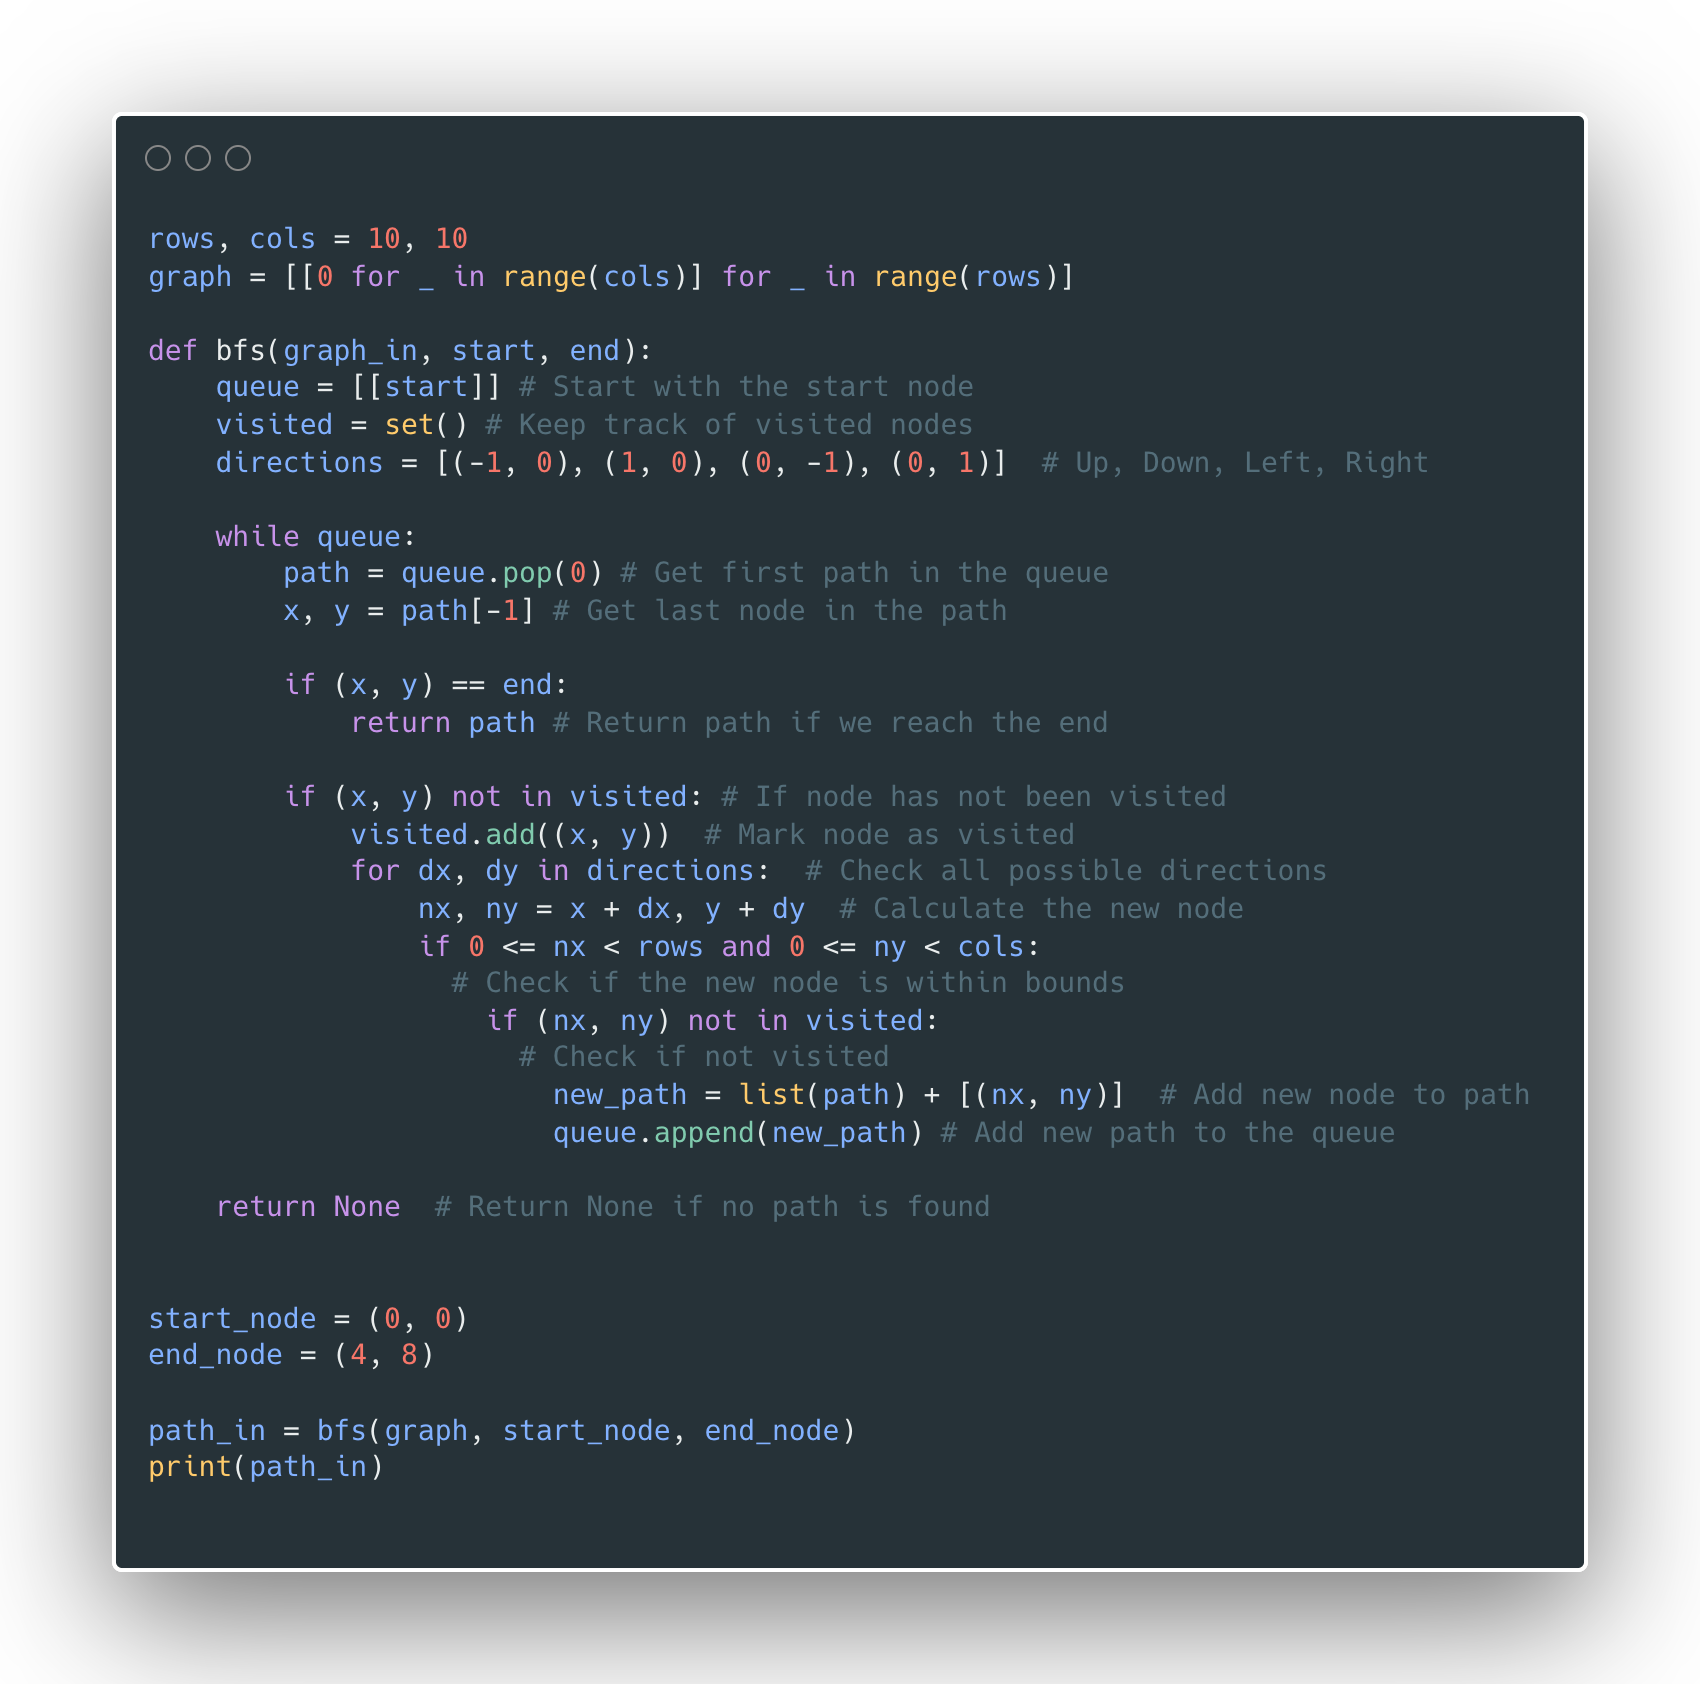
\includegraphics[width=1\linewidth]{Images/Source Code Image (2).png}
    \caption{A coloured screenshot of the code}
\end{figure}
\textbf{}\newline
\newpage

\subsubsection{Prototype details:} 
Currently, the BFS algorithm is working well for 2 defined points: a start and end node. It outputs a basic list of the coordinates that were followed to reach the end node from the start node. However, there is no visualisation as of yet, this will be implemented in the next iteration after some planning. As well as this, the BFS algorithm can currently handle only 2 points at a time, therefore I will be researching into how I can implement more points and allow the user to be able to set points to stop at.
\begin{figure}[htbp]
    \centering
    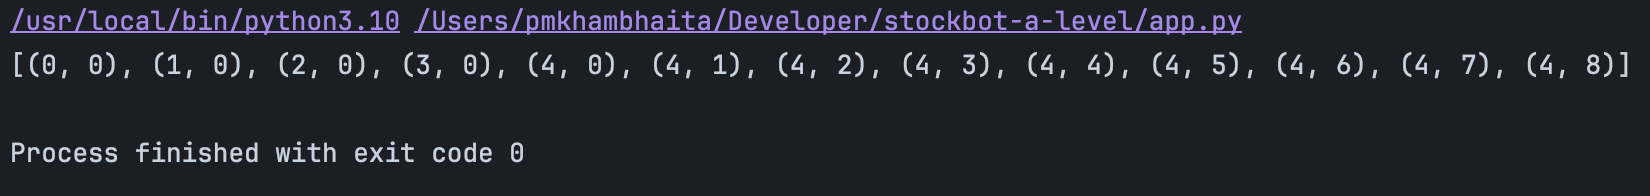
\includegraphics[width=0.8\textwidth]{Images/Screenshot 2025-03-30 at 11.18.52.png}
    \caption{The output of my algorithm with start at (0,0) and end at (4,8)}
\end{figure}

\subsubsection{Testing:}
\begin{table}[htbp]
\centering
\begin{tabularx}{\textwidth}{|l|X|p{3.5cm}|p{3.5cm}|c|}
\hline
\textbf{ID} & \textbf{Description} & \textbf{Expected} & \textbf{Actual} & \textbf{Pass?} \\
\hline
T1.1.1 & Input 0,0 and 9,9 & Direct path between both points & Direct path between points & X \\
\hline
T1.1.2 & Input 1,2 and 5,7 & Direct path between defined points only & Direct path between 1,2 and 5,7 & X \\
\hline
T1.1.3 & Input -1,-1 and 4,8 & Returns error & Error and break & \~{} \\
\hline
T1.1.4 & Input 0,1 and 10,10 & Return error & Error and break & \~{} \\
\hline

\end{tabularx}
\caption{Testing results for iteration 1}
\end{table}

\subsubsection{Tests justification}
These tests were for the main functionality of the program: the BFS must work because it is the heart of my program.
\subsubsection{Fixes}
T1.1.1 and T1.1.2 were successful, meaning the core functionality of the program is functional as expected. However, T1.1.3 and T1.1.4 were partially successful. While I did include the validation, I did not add a graceful error message, it was left to the basic python error-catching mechanisms. This will be fixed in the next iteration.

\newpage

\subsubsection{Screenshots of tests/program}

\begin{figure}[htbp!]
    \centering
    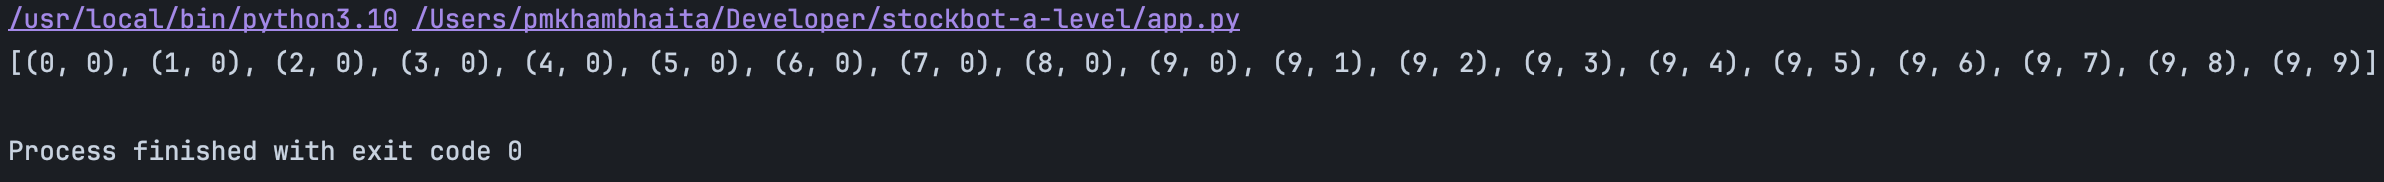
\includegraphics[width=1\linewidth]{Images/t1.1.png}
    \caption{T1.1.1 Output}
    \label{fig:enter-label}
\end{figure}

\begin{figure}[htbp!]
    \centering
    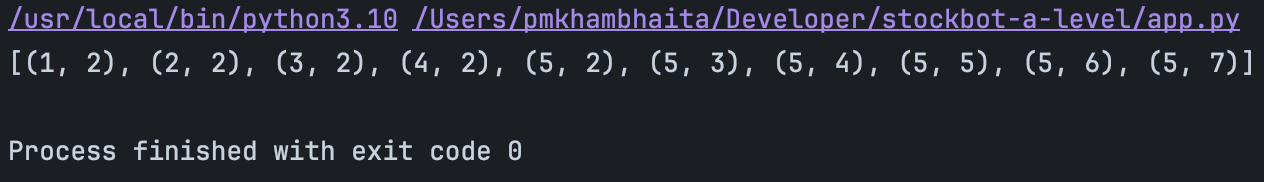
\includegraphics[width=1\linewidth]{Images/t1.2.png}
    \caption{T1.1.2 Output}
    \label{fig:enter-label}
\end{figure}

\begin{figure}[htbp!]
    \centering
    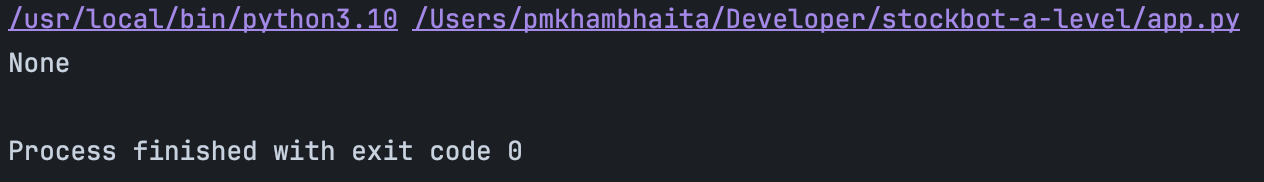
\includegraphics[width=1\linewidth]{Images/t1.3,1.4.png}
    \caption{T1.1.3 Output}
    \label{fig:enter-label}
\end{figure}

\begin{figure}[htbp!]
    \centering
    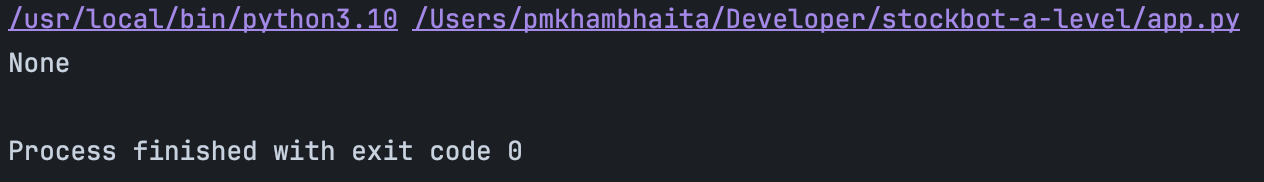
\includegraphics[width=1\linewidth]{Images/t1.3,1.4.png}
    \caption{T1.1.4 Output}
    \label{fig:enter-label}
\end{figure}

\newpage

\subsubsection{Validation:}
\begin{itemize}
    \item Boundary check: I ensured that the new node \verb|(nx, ny)| is within the bounds of the graph
    \item Visited check: I checked that the new node \verb|(nx, ny)| has not been visited before.
\end{itemize}

\subsubsection{Qodana Analysis}
    \begin{itemize}
        \item Issues identified: Shadowed name from outer scope
        \item Resolved issues: Modified variable name to prevent this
    \end{itemize}

\begin{figure}[htbp!]
    \centering
    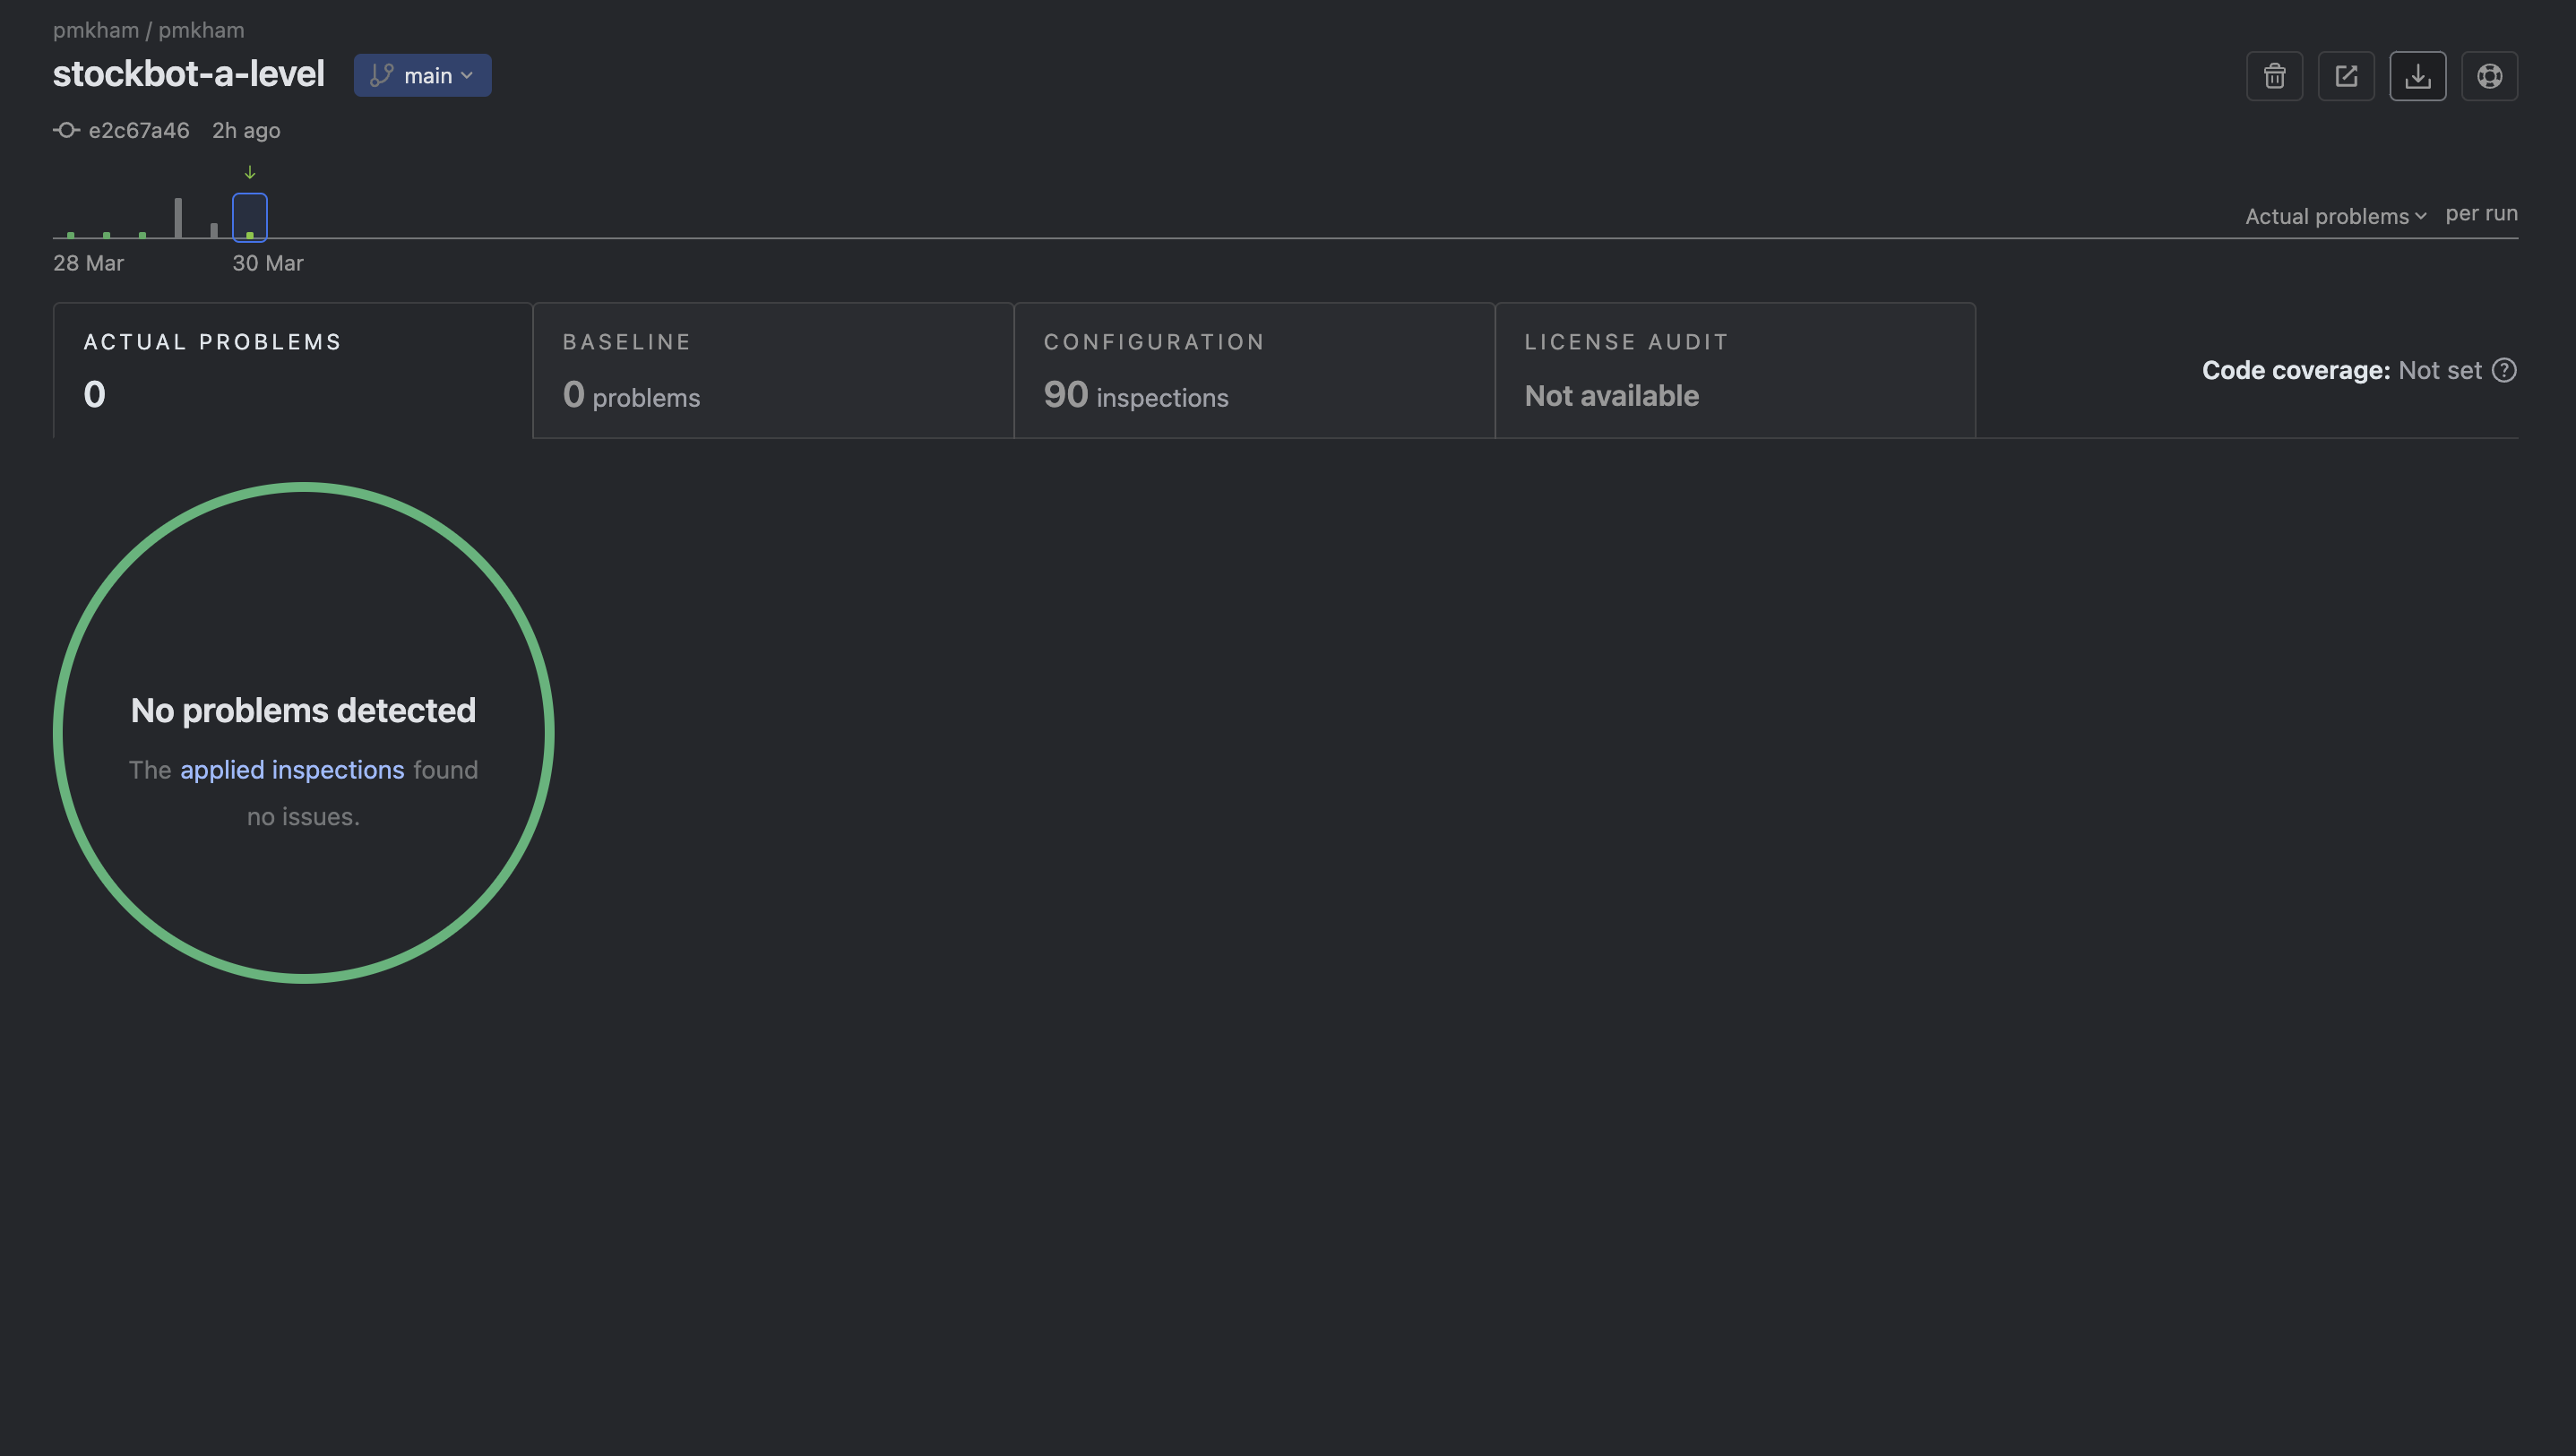
\includegraphics[width=1\linewidth]{Images/qodana-sai1.png}
    \caption{As of commit e2c67a46, no problems were identified.}
\end{figure}

\subsubsection{Review:}
\begin{itemize}
    \item Overall this iteration was quite successful. I managed to get a functional BFS algorithm working between 2 points, however I must be careful in not only validating but adding error messages for specific cases.
    \item Since this is still quite basic, I stuck to a simple procedural format rather than object-oriented principles. In the next iteration, I will be applying object-oriented principles as the program greatens in complexity.
\end{itemize}



\newpage

\subsubsection{Iteration 2: Multi-point BFS and Visualisation}

\textbf{Code Changes:}
\begin{itemize}
    \item \textbf{GitHub Commits:} c90ad6a, 7f76931, 9f2e44b, c88ec49, 94fef19, bc69274, 8081015, 0499de6
    \item \textbf{Modular Structure:}
    \begin{itemize}
        \item I have now implemented an object-oriented approach to the problem, separating each section into their respective classes. Now that my solution is developing in complexity, I decided to separate the elements of my program further into distinct classes, referencing each other when necessary.
    \end{itemize}
\end{itemize}

\textbf{Code Quality:}
\begin{itemize}
    \item \textbf{Annotations added:} I annotated key methods and classes with simple comments as to what they did and any program-specific syntax like my labelling scheme for the visualisation.

    \item \textbf{Modular approach:} I have now implemented an object-oriented approach in my solution, splitting the grid and pathfinder logic into 2 separate classes, referenced by outer functions that process user input and output.
\end{itemize}

\newpage

\subsubsection{Code Implementation:}

\lstinputlisting[style=custompython]{/Users/pmkhambhaita/Documents/GitHub/stockbot-documentation/Code/sa2.py}


\begin{figure}[htbp!]
    \centering
    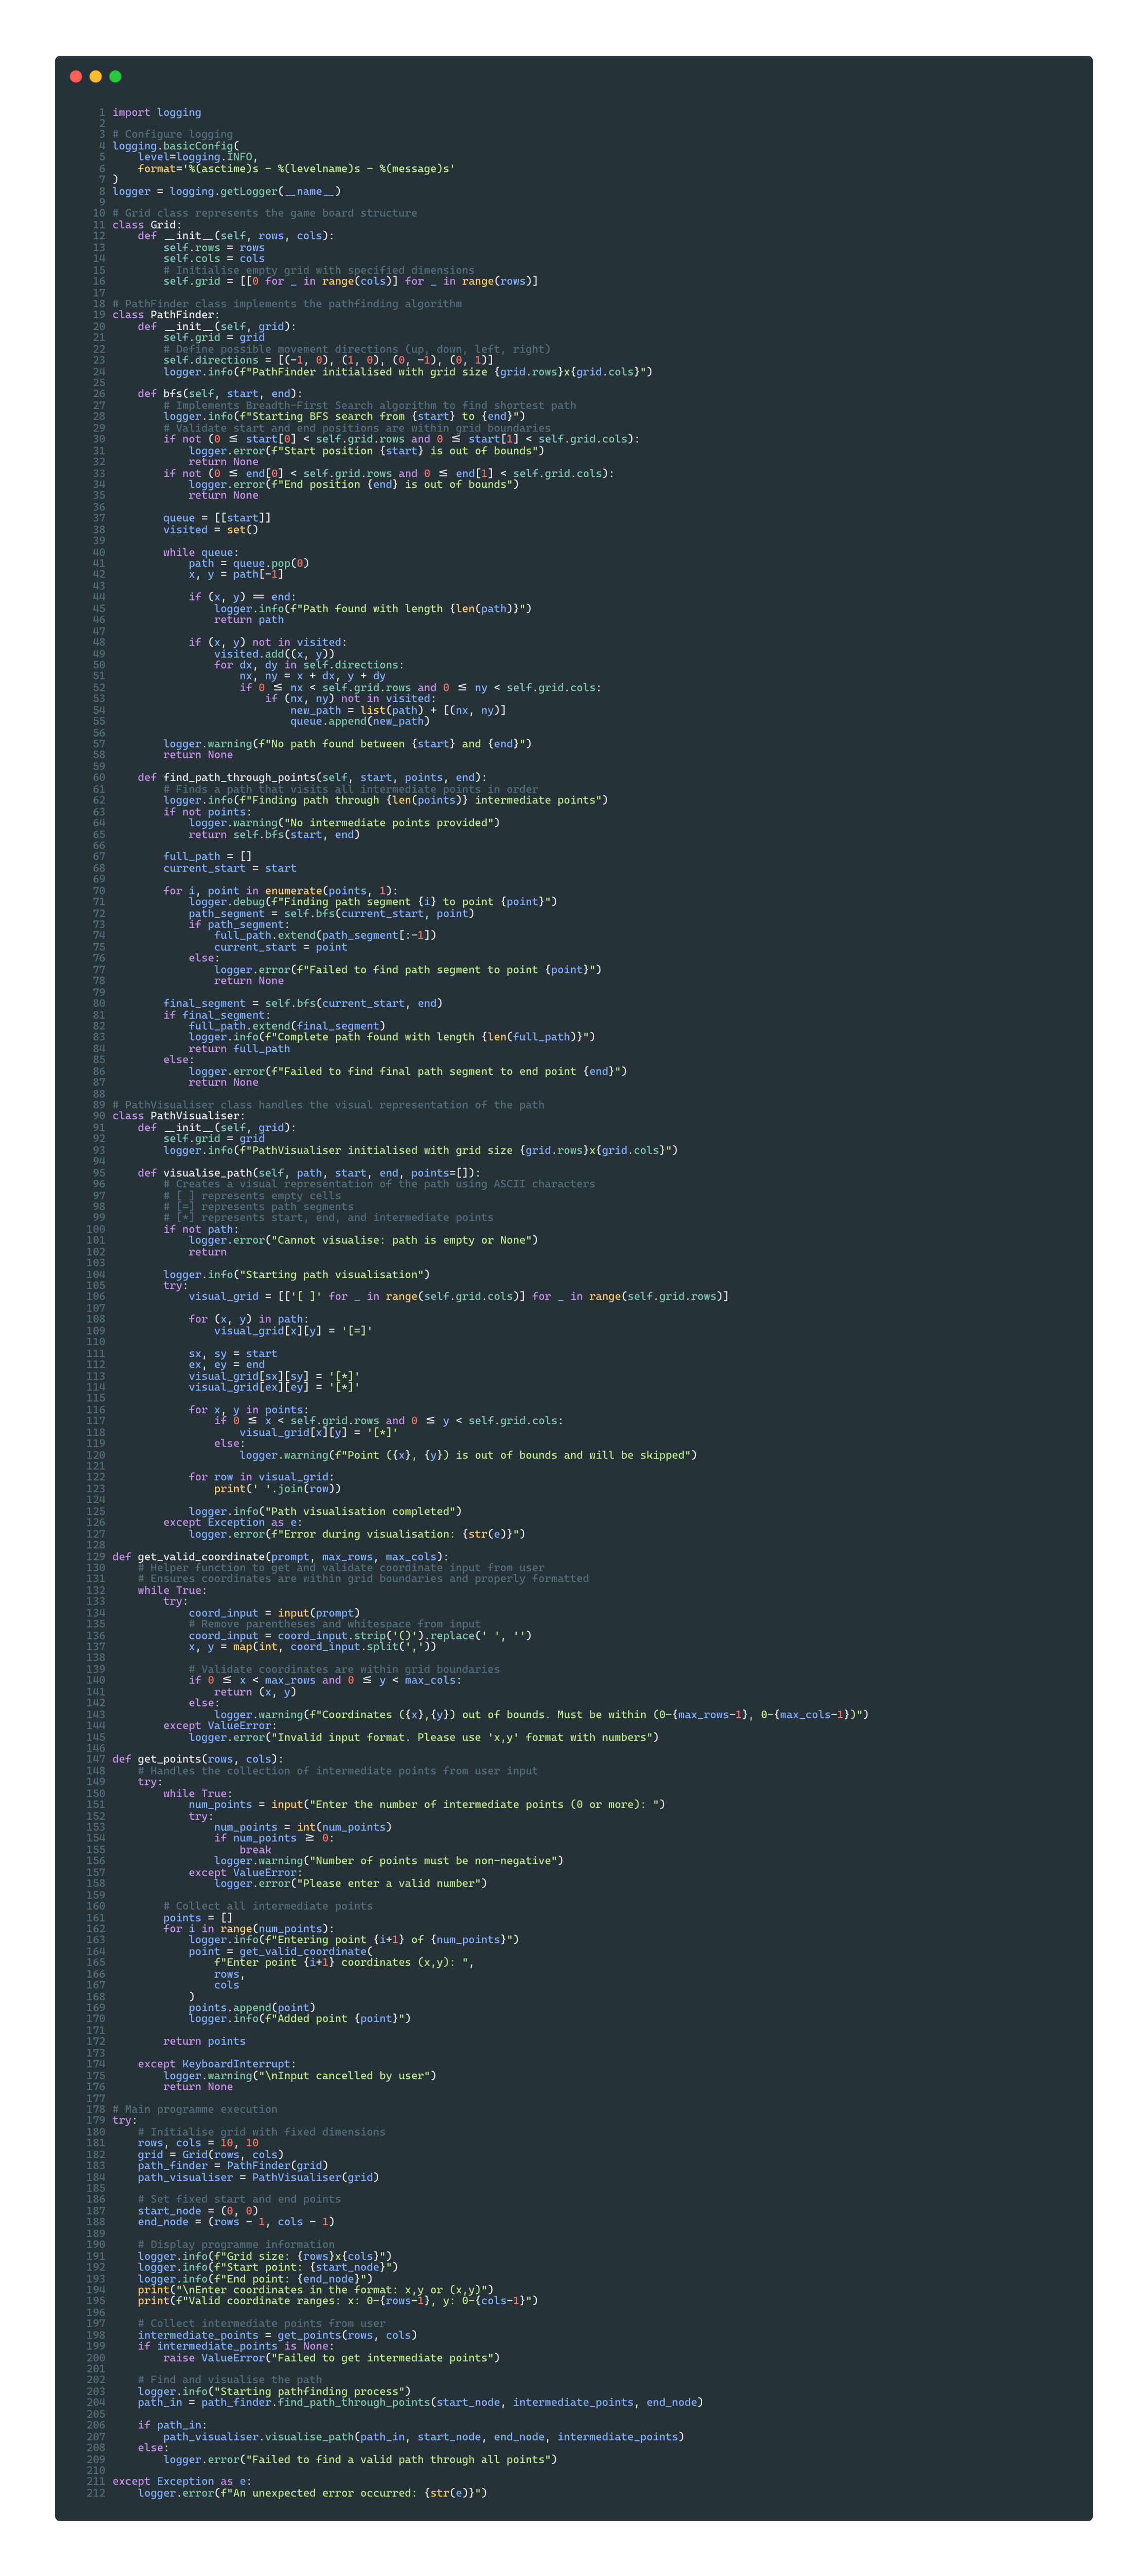
\includegraphics[width=0.61\linewidth]{Images/sa2.png}
    \caption{A coloured screenshot of the code}
\end{figure}
\textbf{}\newline
\newpage

\subsubsection{Prototype details:} 
The BFS algorithm is now working flawlessly, and I added some more debugging features like constant logging and output to the terminal using the \verb|logging| library within python. A timestamp and message is outputted when something of significance happens. The visualisation is also working excellently, and the user input is robust and easy to use. However, I do need to improve some parts of the logging, perhaps including the path the program will trace. As well as this, the path length is slightly inaccurate: it counts the start and end points, meaning it is 1 more than actual.

\begin{figure}[htbp]
    \centering
    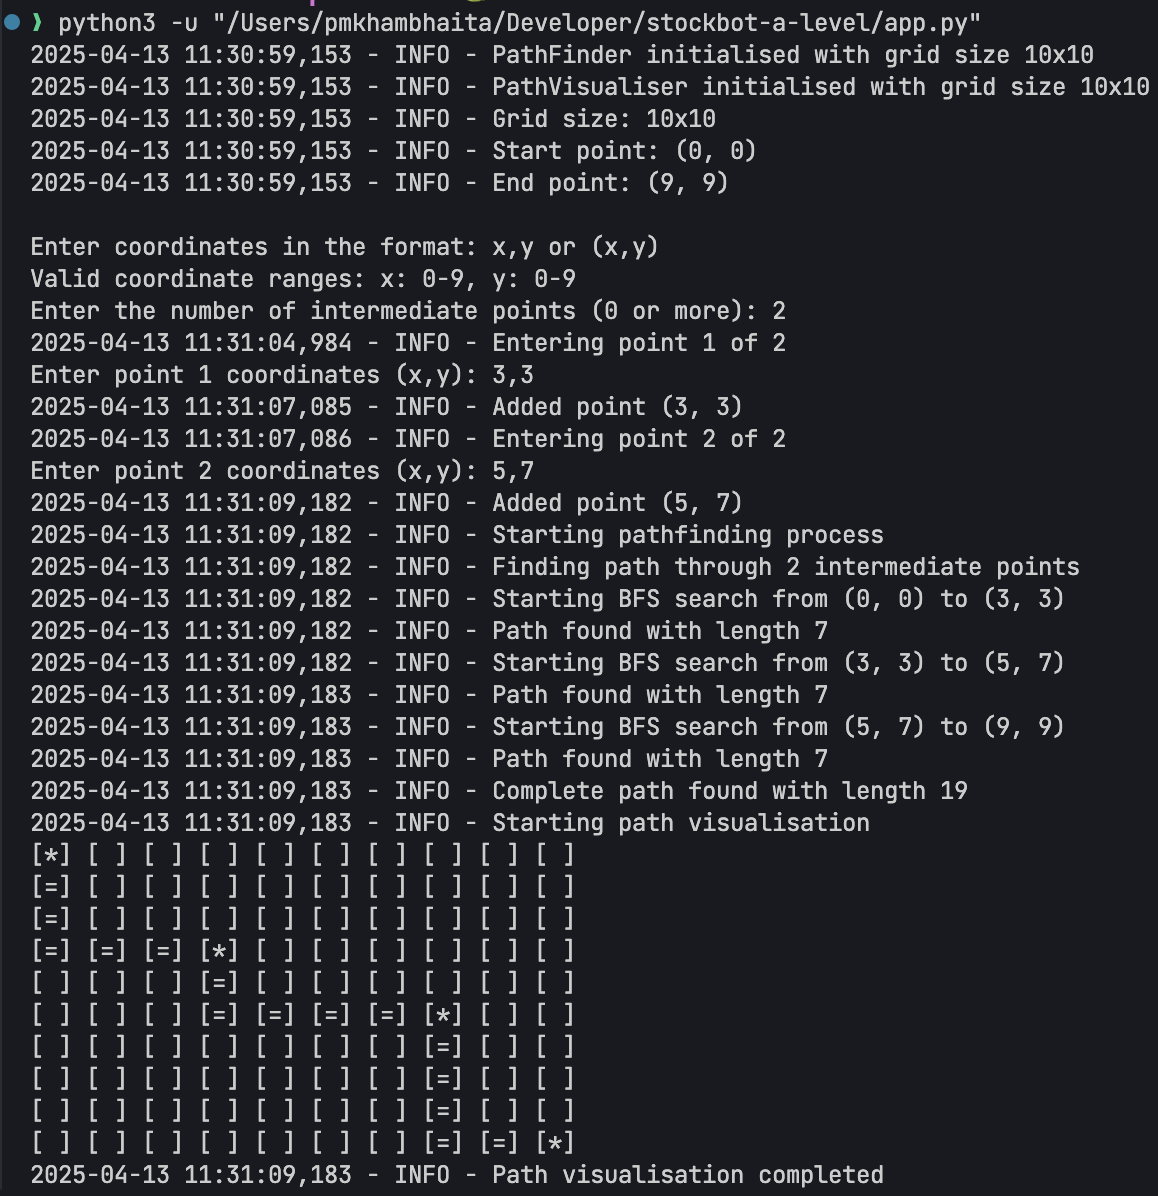
\includegraphics[width=0.8\textwidth]{Images/sa2test1.png}
    \caption{The output of my algorithm with points at (3,3) and end at (5,7)}
\end{figure}

\newpage

\subsubsection{Testing:}
\begin{table}[htbp]
\centering
\begin{tabularx}{\textwidth}{|l|X|p{3.5cm}|p{3.5cm}|c|}
\hline
\textbf{ID} & \textbf{Description} & \textbf{Expected} & \textbf{Actual} & \textbf{Pass?} \\
\hline
T1.2.1 & No intermediate points selected & Direct path between start and end & Direct path between start and end & X \\
\hline
T1.2.2 & Input 3,4 and 5,8 & Direct path between start and end stopping at defined points only & Direct path between start and end stopping at 3,4 and 5,8 & X \\
\hline
T1.2.3 & Input -1,-1 & Returns error & Returned graceful error and allowed retry & X \\
\hline
T1.2.4 & Input one valid and one non-valid point & Return error & Returned graceful error and allowed retry & X \\
\hline
T1.2.5 & Input 5 invalid points & Prevent entering from 1st points & Prevented addition of extra points until valid & X \\
\hline
T1.2.6 & Input valid points and verify it is the shortest path & Shortest path found & Shortest path found, path length incorrect & \~{} \\
\hline

\end{tabularx}
\caption{Testing results for iteration 1}
\end{table}

\subsubsection{Tests justification}
These tests were checking the validation measures I put in place for the SPA. These checked that all the validation was working, from boundary testing to existence validation. This was necessary to ensure the program is robust enough for the stakeholders and to cover all cases.


\subsubsection{Fixes}
Almost all tests were successful, and all previous errors have been resolved. However, the last test - T1.2.6 - was only a partial success - while the path was the shortest, the path length was out by +1. The issue was that the path length was being reported as the number of nodes in the path, but the actual path length should be the number of steps between nodes, which is one less than the number of nodes. Hence, I changed \verb|len(path)| to \verb|len(path) - 1|. This has been fixed in commit 121c011 and 1a7da80.

\newpage

\subsubsection{Screenshots of tests/program}

\begin{figure}[htbp!]
    \centering
    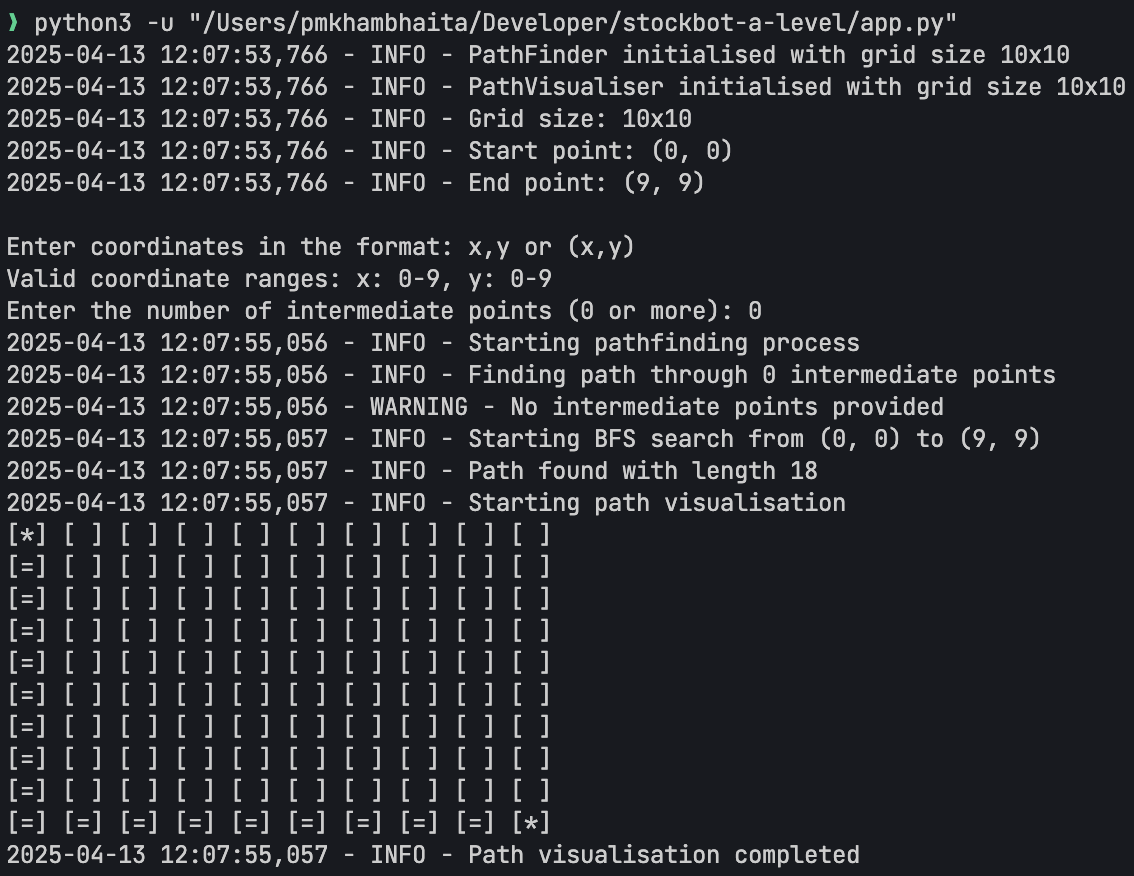
\includegraphics[width=1\linewidth]{Images/t1.2.1.png}
    \caption{T1.2.1 Output}
    \label{fig:enter-label}
\end{figure}

\begin{figure}[htbp!]
    \centering
    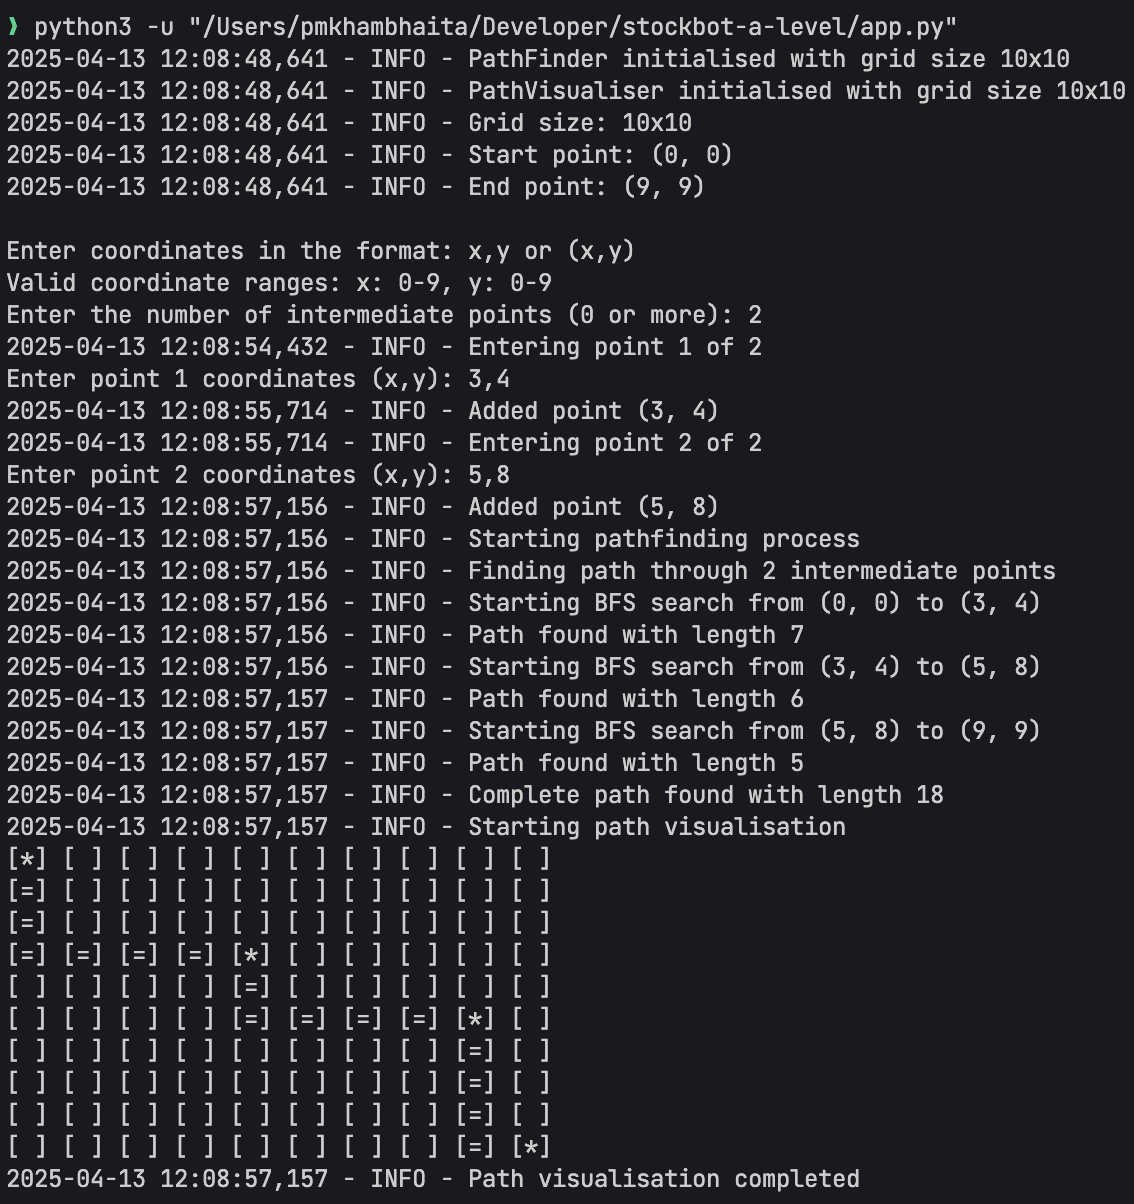
\includegraphics[width=1\linewidth]{Images/t1.2.2.png}
    \caption{T1.2.2 Output}
    \label{fig:enter-label}
\end{figure}

\begin{figure}[htbp!]
    \centering
    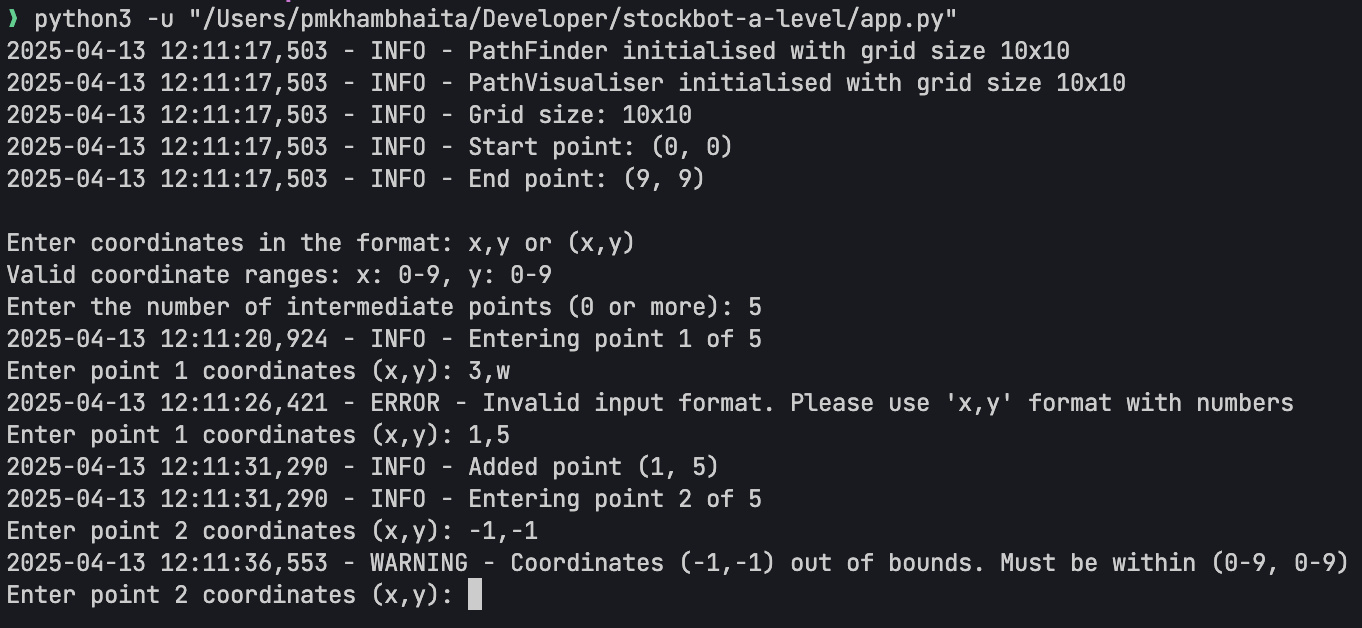
\includegraphics[width=1\linewidth]{Images/t1.2.x.png}
    \caption{T1.2.3/4/5 Output}
    \label{fig:enter-label}
\end{figure}

\begin{figure}[htbp!]
    \centering
    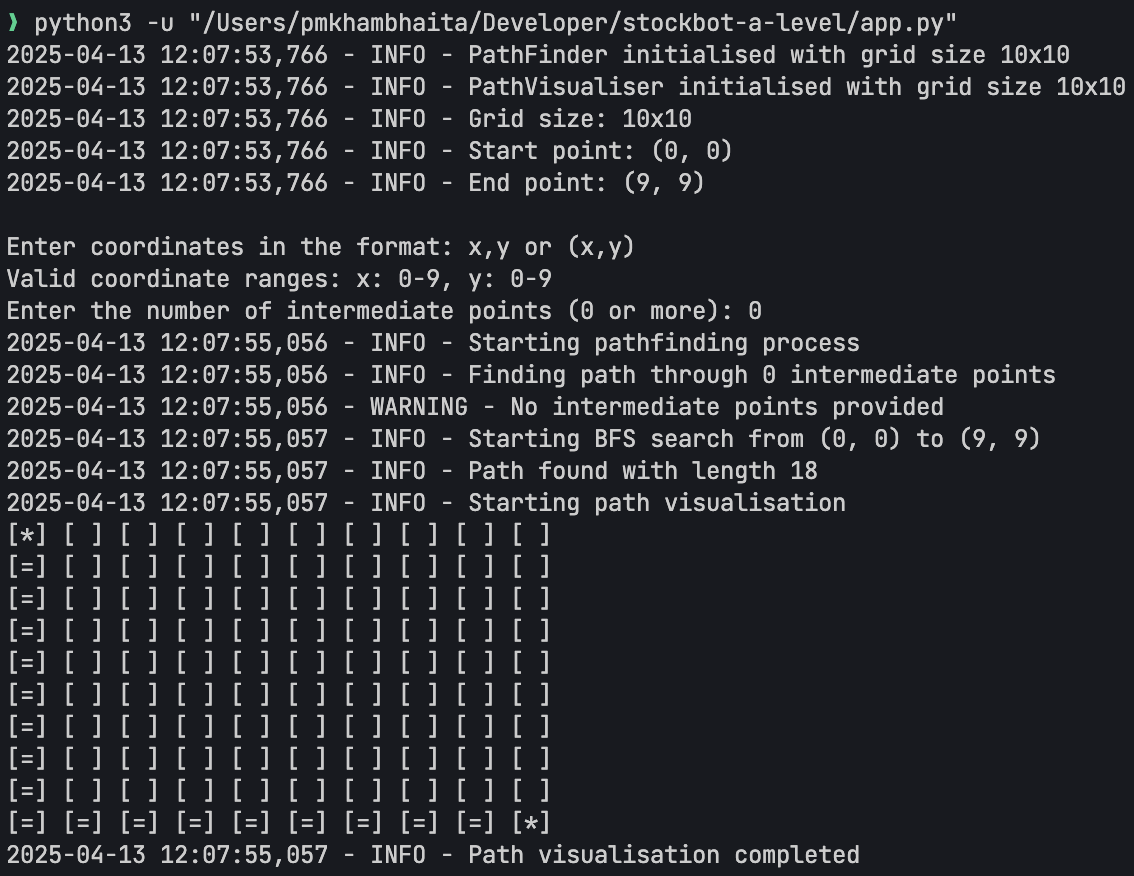
\includegraphics[width=1\linewidth]{Images/t1.2.1.png}
    \caption{T1.2.6 Output (fixed)}
    \label{fig:enter-label}
\end{figure}

\newpage

\subsubsection{Validation:}
\begin{itemize}
    \item \textbf{User input boundary \& range validation} - Confirms all user-provided points are within the grid boundaries and valid range of 0-9.
    \item \textbf{Type \& format validation} - Ensures coordinates are entered in the correct format (x,y) and contain valid numbers
    \item \textbf{Number of points validation} - Checks that the number of intermediate points entered is a non-negative integer
    \item \textbf{Path visualisation validation} - Confirms a path exists before attempting to visualise it
    \item \textbf{User point existence validation} - Handles the case where no intermediate points are provided
    \item \textbf{Exception handling} - Catches and logs any unexpected errors during program execution
\end{itemize}

\subsubsection{Qodana Analysis}
   I resolved all of the issues flagged by Qodana in commit c78f7fc6. Most of the errors were shadwing names from outer scopes, so I used the refactor function in my IDE to fix these issues.

\begin{figure}[htbp!]
    \centering
    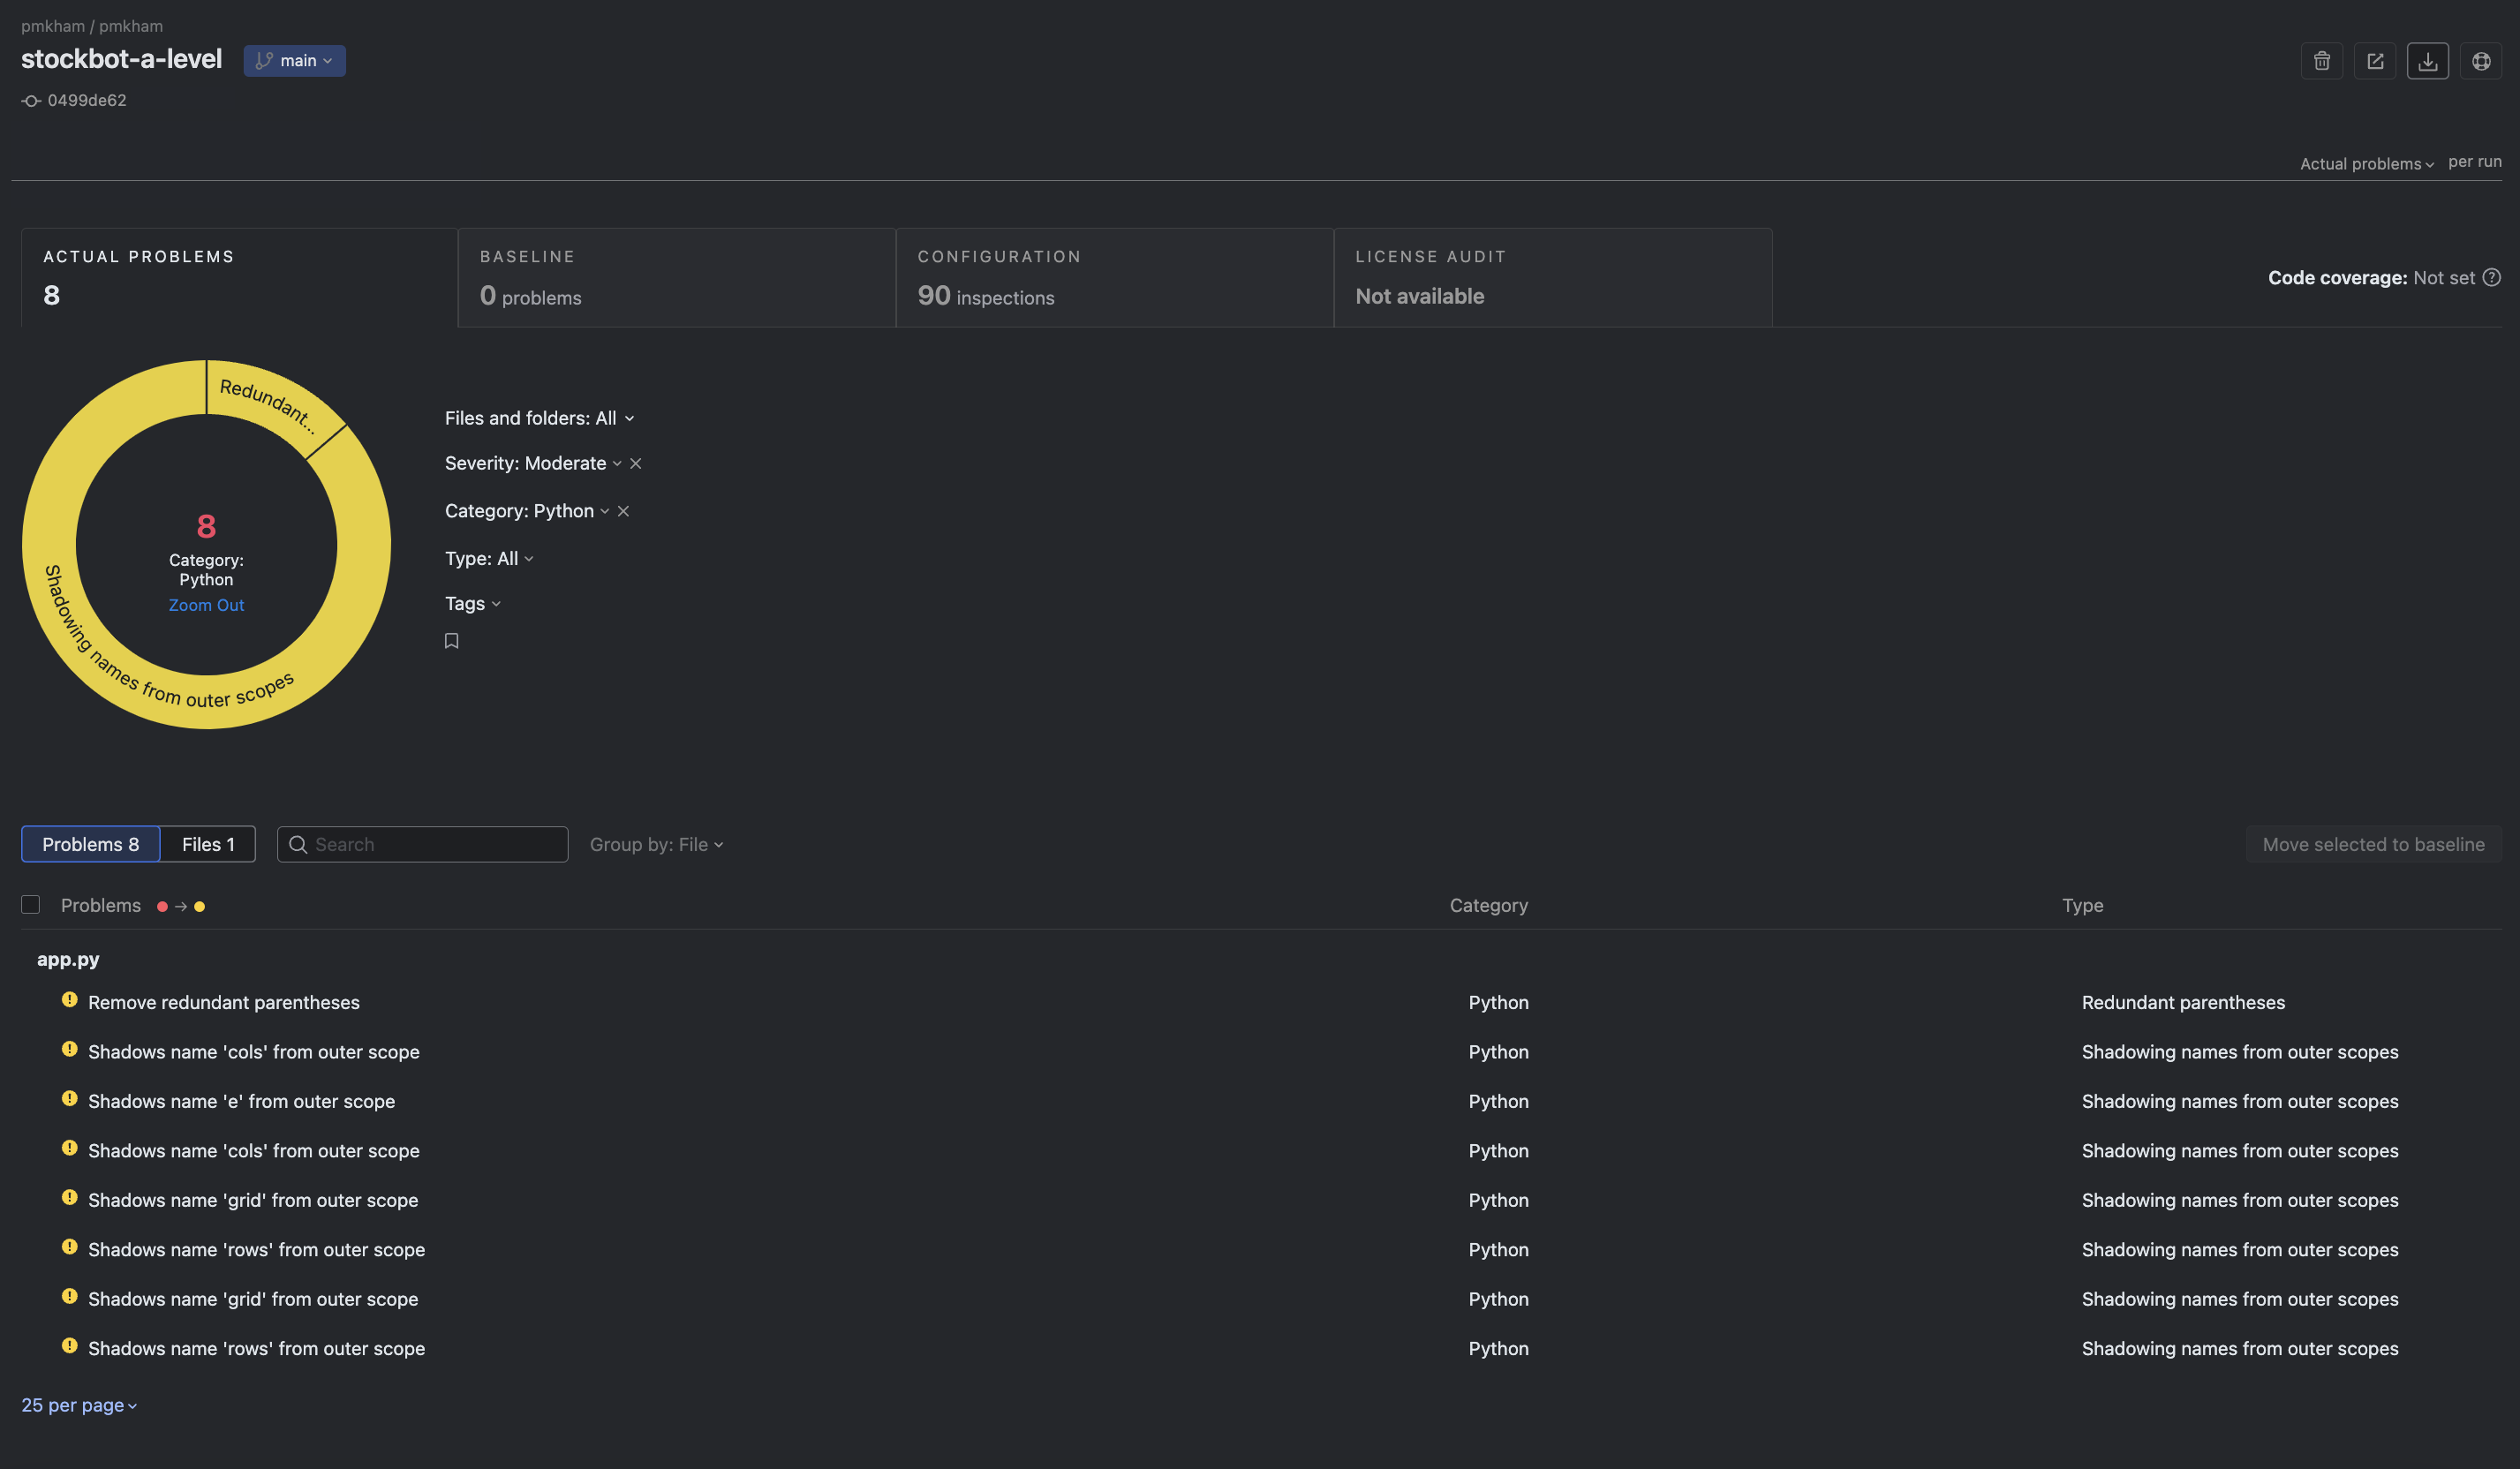
\includegraphics[width=0.85\linewidth]{Images/qodana-sa2.png}
    \caption{As of commit 1a7da80, 8 problems were identified.}
\end{figure}

\subsubsection{Review:}
 Overall this iteration was very successful. I have now completed what I set out to do in this sprint. There were some minor errors along the way, but they were fixed very quickly: they were mainly logic errors rather than syntax.

\clearpage
\subsection{Sprint Review and Retrospective}

\subsubsection{Accomplishments}
\begin{itemize}
    \item Completed OCSP-001 to OCSP-003
    \item  I have now successfully implemented the shortest path feature of my program, and is ready to use. Hence, the first stage of my design - getting a functional SPA running - is complete.
\end{itemize}

\subsubsection{Final testing}

This testing is performed by my stakeholders; they each came up with 1 test they would like to perform in person. This testing  conducted using the data provided in Section x.x.x. In this case, since this program has only implemented the SPA, they will only be using the respective criteria:

\begin{itemize}
\item Grid is 15 x 15
\item Points using random num gen between 0 and 14 (x2): (2,5), (8,9), (10,2) 

\end{itemize}

\begin{table}[htbp]
\centering
\begin{tabularx}{\textwidth}{|l|X|p{3.5cm}|p{3.5cm}|c|}
\hline
\textbf{ID} & \textbf{Description} & \textbf{Expected} & \textbf{Actual} & \textbf{Pass?} \\
\hline
T1.F.1 & Path found using input points & Path between start and end including user-defined points& Direct path between start and end stopping at (2,5), (8,9) and (10,2)  & X \\
\hline
T1.F.2 & Input invalid points (letters, numbers and symbols) & Warns user that points are invalid & Prevents user from entering the points and displays a descriptive message & X \\
\hline
T1.F.3 & Input no points &  Direct path between start and end & Direct path between start and end & X \\
\hline
\end{tabularx}
\end{table}

\subsubsection{Testing Summary}
\begin{table}[htbp]
\centering
\begin{tabular}{|l|c|}
\hline
\textbf{Metric} & \textbf{Count} \\
\hline
Total tests conducted & 13 \\
\hline
Tests passed & 11 \\
\hline
Tests failed & 2 \\
\hline
Fixed issues & 3 \\
\hline
\end{tabular}
\caption{Sprint 1 testing summary}
\end{table}

\newpage

\textbf{Validation}
    \begin{itemize}
    \item \textbf{Grid Boundary Validation for Start/End Points} - Checks if coordinates are within grid dimensions
    \item \textbf{User Input Format Validation} - Validates coordinate input format (x,y)
    \item \textbf{User Input Range Validation} - Confirms coordinates are within valid grid dimensions
    \item \textbf{Number of Points Validation} - Ensures number of intermediate points is non-negative
    \item \textbf{Path Existence Validation} - Verifies if a valid path exists between points
    \item \textbf{Intermediate Point Boundary Validation} - Ensures user-provided points are within grid boundaries
    \item \textbf{Path Visualisation Validation} - Checks if a path exists before attempting visualisation
\end{itemize}

\textbf{Robustness}
\begin{itemize}
    \item \textbf{Exception Handling} -- Uses try-except blocks to catch and log unexpected errors
    \item \textbf{Logging Implementation} -- Comprehensive logging of program flow and errors
    \item \textbf{Default Parameter Values} -- Uses None as default for optional parameters
    \item \textbf{Queue Management in BFS} -- Properly manages the queue in breadth-first search
    \item \textbf{Path Segment Validation} -- Validates each segment of the multi-point path
    \item \textbf{Keyboard Interrupt Handling} -- Catches user interruptions during input collection
    \item \textbf{Consistent Return Values} -- Functions return None for failure cases
    \item \textbf{Empty Points List Handling} -- Gracefully handles cases with no intermediate points
\end{itemize}

\subsubsection{Code Quality Metrics}

    \begin{itemize}
        \item Specific code quality metrics
        \item List of issues resolved with before/after comparisons
        \item Technical debt measurements
    \end{itemize}


\subsubsection{Sprint Review Outcomes}
\begin{itemize}
    \item Specific feedback received
    \item Decisions made for next sprint
\end{itemize}


\clearpage

\section{Final Solution Review}

\subsection{Solution Overview}
Describe the complete solution with reference to requirements from analysis.

\subsection{Code Structure and Modularity}
Explain the final structure with diagrams if helpful.

\subsection{Key Implementation Features}
Highlight innovative or complex aspects of the solution.

\subsection{Comprehensive Validation Strategy}
Summarize the validation approach across the entire project.

\subsection{Maintenance Considerations}
Explain how the code is designed for future maintenance.

